\section{Bloch--Floquet formulation and observables}
\label{sec:bloch}

\subsection{Square lattice and Bloch conditions}
We generate the two-dimensional periodic medium by translating the square cell $\Omega_{\mathrm{cell}}=[0,L]\times[0,L]$ along
\begin{equation}
\bm{a}_1=\begin{bmatrix}L\\0\end{bmatrix},\qquad
\bm{a}_2=\begin{bmatrix}0\\L\end{bmatrix}.
\label{eq:lattice_vectors}
\end{equation}
The corresponding reciprocal vectors satisfy $\bm{a}_i\cdot\bm{b}_j=2\pi\delta_{ij}$:
\begin{equation}
\bm{b}_1=\frac{2\pi}{L}\begin{bmatrix}1\\0\end{bmatrix},\qquad
\bm{b}_2=\frac{2\pi}{L}\begin{bmatrix}0\\1\end{bmatrix}.
\label{eq:reciprocal_vectors}
\end{equation}
The first Brillouin zone is $\mathcal{B}=[-\pi/L,\pi/L]^2$. For the isotropic square lattice, $C_{4v}$ symmetry permits the path $\Gamma(0,0)$--$X(\pi/L,0)$--$M(\pi/L,\pi/L)$--$\Gamma$. Anisotropy reduces the symmetry to $C_{2v}$ for $\theta=0^\circ$ or $90^\circ$, and to $C_2$ at general orientation; full-zone measures are therefore evaluated over the corresponding Brillouin zone.

\begin{figure*}[!tbp]
\centering
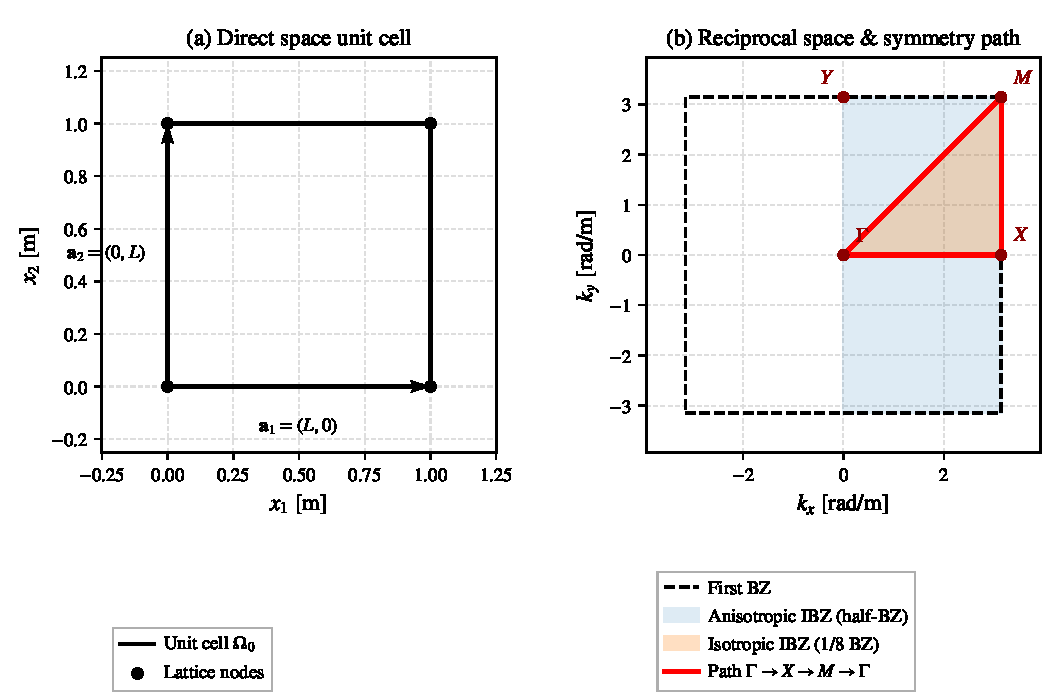
\includegraphics[width=\textwidth]{figures/fig02_lattice_ibz.pdf}
\caption{(a) Square periodic lattice. (b) First Brillouin zone and the high-symmetry contour $\Gamma$--$X$--$M$--$\Gamma$.}
\label{fig:lattice_ibz}
\end{figure*}

For a time-harmonic displacement $\bmu(\bmx,t)=\tilde{\bmu}(\bmx)e^{\iu(\bmk\cdot\bmx-\omega t)}$, Bloch periodicity gives
\begin{equation}
\bmu(\bmx+\bm{a}_\alpha)=\bmu(\bmx)e^{\iu\bmk\cdot\bm{a}_\alpha},\qquad \alpha\in\{1,2\}.
\label{eq:bloch_displacement}
\end{equation}
Because the approximation is $C^1$-conforming, differentiating the displacement relation gives:
\begin{equation}
\frac{\partial\bmu}{\partial x_\beta}(\bmx+\bm{a}_\alpha)=\frac{\partial\bmu}{\partial x_\beta}(\bmx)e^{\iu\bmk\cdot\bm{a}_\alpha},\qquad
\frac{\partial^2\bmu}{\partial x_1\partial x_2}(\bmx+\bm{a}_\alpha)=\frac{\partial^2\bmu}{\partial x_1\partial x_2}(\bmx)e^{\iu\bmk\cdot\bm{a}_\alpha}.
\label{eq:bloch_derivatives}
\end{equation}
Thus displacement, first derivatives, and cross derivatives all take the same Bloch phase; a different phase for derivative degrees of freedom would break $C^1$ continuity across cell boundaries.

\subsection{Nondimensionalization}
For Case~H, we scale length, frequency, and velocity with the cell length $L$, shear modulus $\mu$, and density $\rho$:
\begin{equation}
\bark=\frac{kL}{\pi},\qquad \barw=\frac{\omega}{\omega_0},\qquad
\omega_0=\sqrt{\frac{\mu}{\rho L^2}},\qquad
\bar{l}_m=\frac{l_m}{L},\qquad
\ellbar=\frac{\ell_{\mathrm{i}}}{L},\qquad
\bar{v}_p=\frac{\omega/k}{\sqrt{\mu/\rho}}.
\label{eq:nondim_defs}
\end{equation}
This gives $c_T=1$ and $c_L=\sqrt{(\lambda+2\mu)/\mu}=\sqrt{3}$ for $\lambda/\mu=1$ ($\nu=0.25$). Case~C uses the matrix shear speed and frequency scale specified in Table~\ref{tab:case_params}.

\subsection{Gap and steering measures}
At each wave vector, the eigenfrequencies are ordered as $\barw_1(\bmk)\le\barw_2(\bmk)\le\cdots$. We distinguish gaps evaluated on one path leg, the complete high-symmetry path, and the full Brillouin zone:
\begin{enumerate}[label=(\alph*)]
  \item \textbf{Leg gap:} for bands $n$ and $n+1$, $\Delta[\mathrm{leg}]=\min_{\bmk\in\mathrm{leg}}\barw_{n+1}(\bmk)-\max_{\bmk\in\mathrm{leg}}\barw_n(\bmk)$; $\Delta_{GX}$ denotes the $\Gamma$--$X$ leg.
  \item \textbf{Path gap:}
  \begin{equation}
  \Delta_{\mathrm{path}}=\min_{\bmk\in\mathrm{path}}\barw_{n+1}(\bmk)-\max_{\bmk\in\mathrm{path}}\barw_n(\bmk).
  \label{eq:delta_path}
  \end{equation}
  \item \textbf{Complete gap:}
  \begin{equation}
  \Delta_{\mathrm{complete}}=\min_{\bmk\in\mathcal{B}}\barw_{n+1}(\bmk)-\max_{\bmk\in\mathcal{B}}\barw_n(\bmk).
  \label{eq:delta_complete}
  \end{equation}
\end{enumerate}
Since the leg, path, and full zone are nested sets, $\Delta[\mathrm{leg}]\ge\Delta[\mathrm{path}]\ge\Delta[\mathrm{complete}]$:
\begin{equation}
\Delta[\mathrm{leg}]\ge\Delta[\mathrm{path}]\ge\Delta[\mathrm{complete}].
\label{eq:gap_hierarchy}
\end{equation}
A positive leg gap indicates directional filtering; a complete band gap requires $\Delta_{\mathrm{complete}}>0$.

The orientation sensitivity of a directional gap is measured by
\begin{equation}
S_\theta=\frac{\max_\theta\left|\frac{\partial\Delta}{\partial\theta}\right|}{\max_\theta\Delta}\quad[\mathrm{rad}^{-1}].
\label{eq:S_theta_def}
\end{equation}
The group velocity and its angular deviation from the wave vector are
\begin{equation}
\bmv_g=\nabla_{\bmk}\omega.
\label{eq:group_velocity}
\end{equation}
\begin{equation}
\delta=\angle\bmv_g-\angle\bmk.
\label{eq:steering_angle}
\end{equation}
